\subsection{x86: \IFRU{3 аргумента}{3 arguments}}

\subsubsection{MSVC}

\IFRU{Компилируем при помощи MSVC 2010 Express, и в итоге получим:}
{Let's compile it by MSVC 2010 Express and we got:}

\begin{lstlisting}
$SG3830	DB	'a=%d; b=%d; c=%d', 00H

...

	push	3
	push	2
	push	1
	push	OFFSET $SG3830
	call	_printf
	add	esp, 16					; 00000010H
\end{lstlisting}

\IFRU{Все почти то же, за исключением того, что теперь видно, что аргументы для \printf заталкиваются в стек в обратном порядке: самый первый аргумент заталкивается последним.}
{Almost the same, but now we can see the \printf arguments are pushing into stack in reverse order: and the first argument is pushing in as the last one.}

\IFRU{Кстати, вспомним что переменные типа \Tint в 32-битной системе, как известно, имеет ширину 32 бита, это 4 байта}
{By the way, variables of \Tint type in 32-bit environment has 32-bit width that is 4 bytes}.

\IFRU{Итак, у нас всего 4 аргумента. $4*4 = 16$ ~--- именно 16 байт занимают в стеке указатель на строку плюс еще 3 числа типа \Tint.}
{So, we got here 4 arguments. $4*4 = 16$~---they occupy exactly 16 bytes in the stack: 32-bit pointer to string and 3 number of \Tint type.}

\index{x86!\Instructions!ADD}
\index{x86!\Registers!ESP}
\index{cdecl}
\IFRU{Когда при помощи инструкции \TT{``ADD ESP, X''} корректируется \glslink{stack pointer}{указатель стека} \ESP 
после вызова какой-либо функции, зачастую можно сделать вывод о том, сколько аргументов 
у вызываемой функции было, разделив X на 4.}
{When \gls{stack pointer} (the \ESP register) is corrected by \TT{``ADD ESP, X''}
instruction after a function 
call, often, the number of function arguments could be deduced here: just divide X by 4.}

\IFRU{Конечно, это относится только к cdecl-методу передачи аргументов через стек.}
{Of course, this is related only to \IT{cdecl} calling convention.}

\IFRU{См. также в соответствующем разделе о способах передачи аргументов через стек}
{See also section about calling conventions}~(\ref{sec:callingconventions}).

\IFRU{Иногда бывает так, что подряд идут несколько вызовов разных функций, 
но стек корректируется только один раз, после последнего вызова:}
{It is also possible for compiler to merge several \TT{``ADD ESP, X''} instructions into one, after last call:}

\begin{lstlisting}
push a1
push a2
call ...
...
push a1
call ...
...
push a1
push a2
push a3
call ...
add esp, 24
\end{lstlisting}

\subsubsection{MSVC \AndENRU \olly}
\index{\olly}

\IFRU{Попробуем этот же пример в}{Now let's try to load this example in} \olly.
\IFRU{Это один из наиболее популярных win32-отладчиков user-режима}{It is one of the most 
popular user-land win32 debugger}.
\IFRU{Мы можем компилировать наш пример в}{We can try to compile our example in} MSVC 2012 
\IFRU{с опцией}{with} \TT{/MD} \IFRU{что означает, линковать с библиотекой}{option, meaning, to link 
against} \TT{MSVCR*.DLL},
\IFRU{чтобы импортируемые ф-ции были хорошо видны в отладчике}{so we will able to see imported 
functions clearly in debugger}.

\IFRU{Затем загружаем исполняемый файл в}{Then load executable in} \olly.
\IFRU{Самый первый брякпойнт в}{The very first breakpoint is in} \TT{ntdll.dll}, \IFRU{нажмите}{press} 
F9 (\IFRU{запустить}{run}).
\IFRU{Второй брякпойнт в}{The second breakpoint is in} \ac{CRT}-\IFRU{коде}{code}.
\IFRU{Теперь мы должны найти ф-цию}{Now we should find} \main\EN{ function}.

\IFRU{Найдите этот код скроллируя окно кода до самого верха (MSVC располагает ф-цию \main в самом начале
секции кода)}{Find this code by scrolling the code to the very bottom (MSVC allocates \main function at
the very beginning of the code section)}: 
\figname \ref{fig:printf3_olly_1}.

\IFRU{Кликните на инструкции}{Click on} \TT{PUSH EBP}\IFRU{, нажмите}{ instruction, press} F2 
(\IFRU{установка брякпойнта}{set breakpoint}) \IFRU{и нажмите}{and press} F9 (\IFRU{запустить}{run}).
\IFRU{Нам нужно произвести все эти манипуляции, чтобы пропустить \ac{CRT}-код, потому что нам он пока
не интересен}{We need to do these manupulations in order to skip \ac{CRT}-code, because, we don't really 
interesting in it yet}.

\IFRU{Нажмите}{Press} F8 (\stepover) 6 \IFRU{раз, т.е., пропустить
6 инструкций}{times, i.e., skip 6 instructions}: \figname \ref{fig:printf3_olly_2}.

\IFRU{Теперь}{Now the} \PC \IFRU{указывает на инструкцию}{points to the}
\TT{CALL printf}\EN{ instruction}.
\olly, \IFRU{как и другие отладчики, подсвечивает регистры со значениями, которые изменились}
{like other debuggers, highlights value of registers which were changed}.
\IFRU{Так что, каждый раз, когда мы нажимаем}{So each time you press F8}, \EIP 
\IFRU{изменяется и его значение подсвечивается красным}{is changing and its value looking red}.
\ESP \IFRU{также меняется, потому что значения заталкиваются в стек}{is changing as well, 
because values are pushed into the stack}.

\IFRU{Где находятся эти значения в стеке}{Where are the values in the stack}?
\IFRU{Посмотрите на правое/нижнее окно в отладчике}{Take a look into right/bottom window of debugger}:

\begin{figure}[H]
\centering
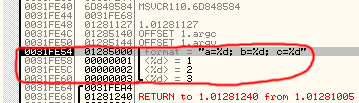
\includegraphics[scale=0.66]{patterns/03_printf/olly3_stack.png}
\caption{\olly: \IFRU{стек, после того как значения там сохранены}{stack after values pushed}
(\IFRU{я сделал здесь округлую красную пометку в графическом редакторе}{I made round red mark 
here in graphics editor})}
\end{figure}

\IFRU{Так что здесь видно 3 столбца: адрес в стеке, значение в стеке и еще дополнительный комментарий
от \olly}{So we can see there 3 columns: address in the stack, 
value in the stack and some additional \olly comments}. 
\olly \IFRU{понимает}{understands} \printf\IFRU{-строки}{-like strings}, 
\IFRU{так что он показывает здесь и строку и 3 значения \IT{привязанных} к ней}{so it reports the 
string here and 3 values \IT{attached} to it}.

\IFRU{Нажмите}{Press} F8 (\stepover).

\IFRU{В коносил мы видим вывод}{In the console we'll see the output}:

\begin{figure}[H]
\centering
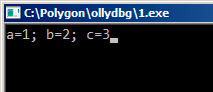
\includegraphics[scale=0.66]{patterns/03_printf/olly3_console.png}
\caption{\RU{Ф-ция }\printf \IFRU{исполнилась}{function executed}}
\end{figure}

\IFRU{Посмотрим, как изменились регистры и состояние стека}{Let's see how registers and stack state 
are changed}: \figname \ref{fig:printf3_olly_3}.

\RU{Регистр }\EAX \IFRU{теперь содержит}{register now contains} \TT{0xD} (13).
That's correct, \printf returns number of characters printed.
\RU{Значение }\EIP \IFRU{изменилось: действительно, теперь здесь адрес инструкции после}
{value is changed: indeed, now there is address of the instruction after} \TT{CALL printf}.
\RU{Значения регистров }\ECX \AndENRU \EDX \IFRU{также изменились}{values are changed as well}.
\IFRU{Очевидно, внутренности ф-ции \printf используют их для каких-то своих нужд}{Apparently, 
\printf function's hidden machinery used them for its own needs}.

\IFRU{Очень важный момент в том что значение \ESP не изменилось. И состояние стека также!}
{A very important thing is that \ESP value is not changed. And stack state too!}
\IFRU{Мы ясно видим здесь и строку формата и соответствующие ей 3 значения, они все еще здесь}
{We clearly see that format string and corresponding 3 values are still there}.
\IFRU{Действительно, по соглашению вызовов \IT{cdecl}, вызывающая ф-ция не очищает аргументы из стека}
{Indeed, that's \IT{cdecl} calling convention, calling function doesn't clear arguments in stack}.
\IFRU{Это должна делать вызывающая ф-ция}{It's caller's duty to do so}.

\IFRU{Нажмите}{Press} F8 \IFRU{снова, чтобы исполнилась инструкция}{again to execute} 
\TT{ADD ESP, 10}\EN{ instruction}: \figname \ref{fig:printf3_olly_4}.

\ESP \IFRU{изменился, но значения все еще в стеке}{is changed, but values are still in the stack}!
\IFRU{Конечно, никому не нужно заполнять эти значения нулями или что-то в этом роде}{Yes, 
of course, no one needs to fill these values by zero or something like that}.
\IFRU{Потому что всё что выше указателя стека}{Because, everything above stack pointer} (\SP) 
\IFRU{это}{is} \IT{\IFRU{шум}{noise}} \OrENRU \IT{\IFRU{мусор}{garbage}}, \IFRU{это всё не имеет
особой ценности}{it has no value at all}.
\IFRU{Было бы очень затратно по времени очищать ненужные элементы стека, к тому же, никому это и не 
нужно}{It would be time consuming to clear unused stack entries, besides, no one really needs to}.

\begin{figure}[H]
\centering
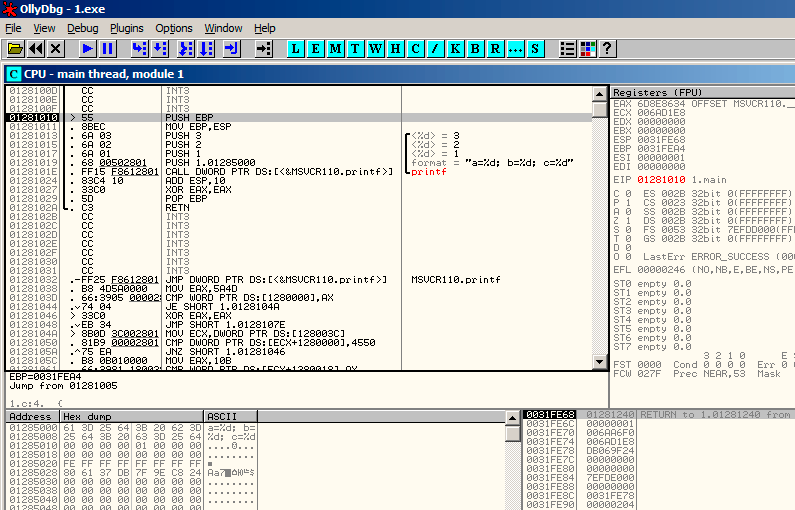
\includegraphics[scale=0.66]{patterns/03_printf/olly3_1.png}
\caption{\olly: \IFRU{самое начало ф-ции}{the very start of the} \main\EN{ function}}
\label{fig:printf3_olly_1}
\end{figure}

\begin{figure}[H]
\centering
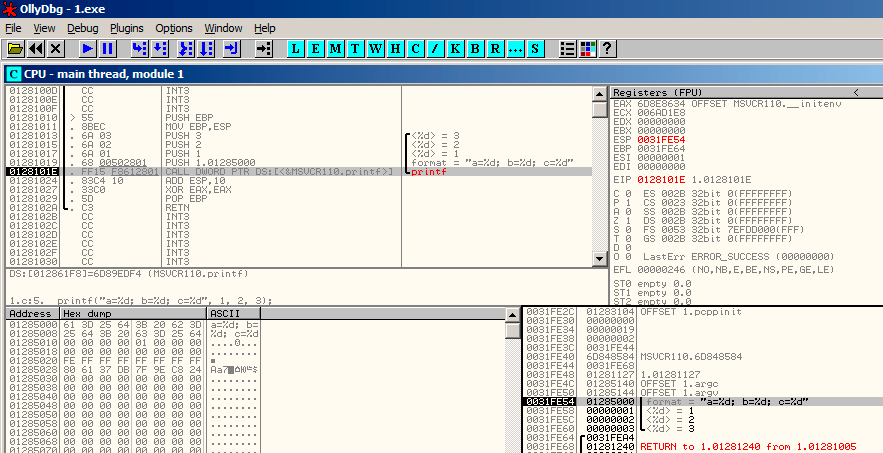
\includegraphics[scale=0.66]{patterns/03_printf/olly3_2.png}
\caption{\olly: \IFRU{перед исполнением}{before} \printf\EN{ execution}}
\label{fig:printf3_olly_2}
\end{figure}

\begin{figure}[H]
\centering
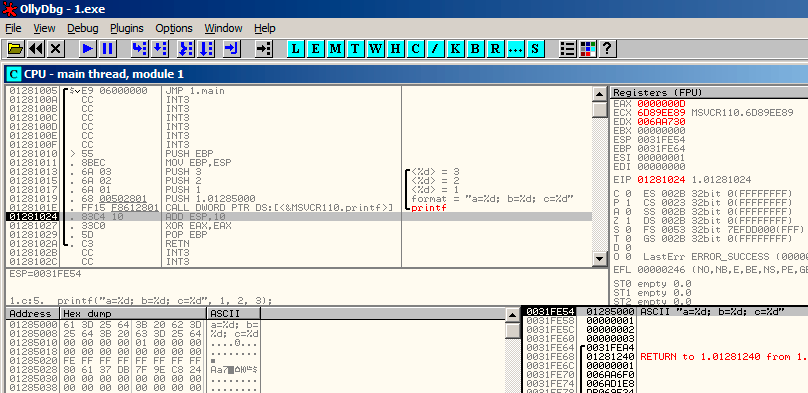
\includegraphics[scale=0.66]{patterns/03_printf/olly3_3.png}
\caption{\olly: \IFRU{после исполнения}{after} \printf\EN{ execution}}
\label{fig:printf3_olly_3}
\end{figure}

\begin{figure}[H]
\centering
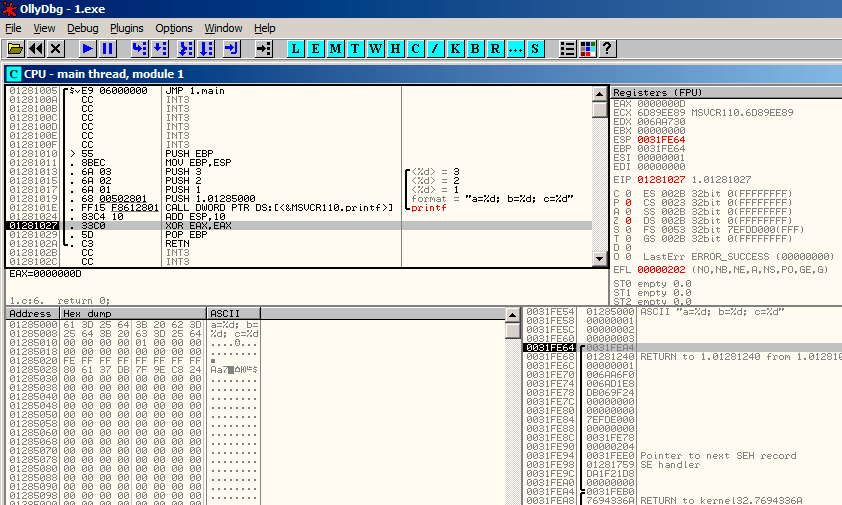
\includegraphics[scale=0.66]{patterns/03_printf/olly3_4.png}
\caption{\olly: \IFRU{после исполнения инструкции}{after} \TT{ADD ESP, 10}\EN{ instruction execution}}
\label{fig:printf3_olly_4}
\end{figure}

\subsubsection{GCC}

\IFRU{Скомпилируем то же самое в Linux при помощи GCC 4.4.1 и посмотрим в \IDA что вышло:}
{Now let's compile the same in Linux by GCC 4.4.1 and take a look in \IDA what we got:}

\begin{lstlisting}
main            proc near

var_10          = dword ptr -10h
var_C           = dword ptr -0Ch
var_8           = dword ptr -8
var_4           = dword ptr -4

                push    ebp
                mov     ebp, esp
                and     esp, 0FFFFFFF0h
                sub     esp, 10h
                mov     eax, offset aADBDCD ; "a=%d; b=%d; c=%d"
                mov     [esp+10h+var_4], 3
                mov     [esp+10h+var_8], 2
                mov     [esp+10h+var_C], 1
                mov     [esp+10h+var_10], eax
                call    _printf
                mov     eax, 0
                leave
                retn
main            endp
\end{lstlisting}

\IFRU{Можно сказать, что этот короткий код, созданный GCC, отличается от кода MSVC только способом помещения 
значений в стек.
Здесь GCC снова работает со стеком напрямую без \PUSH/\POP.}
{It can be said, the difference between code by MSVC and GCC is only in method of placing arguments on the stack.
Here GCC working directly with stack without \PUSH/\POP.}
